%%******************************************************************************
%%
%% pesqbib.tex
%%
%%******************************************************************************
%%
%% Title......: Introduction
%%
%% Author.....: GSCAR-DFKI
%%
%% Started....: Nov 2013
%%
%% Emails.....: renan028@gmail.com
%%
%% Address....: Universidade Federal do Rio de Janeiro
%%              Caixa Postal 68.504, CEP: 21.945-970
%%              Rio de Janeiro, RJ - Brasil.
%%
%%******************************************************************************


%%******************************************************************************
%% SECTION - Pesquisa Técnica
%%******************************************************************************



%%%%%%%%%%%%%%

\subsection{Sensores de Contato}

Visando a medição do contato entre a \emph{Garra Pescadora} e o \emph{Stoplog} foram pesquisados os seguintes sistemas de sensoriamento: sensor de força, sensor indutivo de proximidade,  sensor capacitivo de proximidade. Em sequência foi realizada a
 pesquisa por fornecedores que atendam aos requisitos de projeto.
 

%%%%%%%%%%%%%%

\subsubsection{Sensor de força}

 Sensores de força podem ser utilizados para detectarem a presença da garra pescadora. A análise quantitativa e comparativa dessas forças pode indicar encaixe mal ou bem sucedido durante a operação e, portanto, é considerada uma solução viável mediante calibração. Os diversos tipos de sensores de força e suas aplicações podem ser consultados em \textbf{Guide to the Measurement of Force}, publicado por \textbf{The Institute of Measurement and Control, London}.

 O sensor de força é composto por um transdutor, que é submetido à força, e uma instrumentação associada, responsável por alimentar o transdutor e processar a saída. O transdutor é um dispositivo que recebe um estímulo físico, como a contração elástica do material devido ao peso, e traduz em outra medida física, como variação de voltagem ou corrente elétrica. Esta variação obedece uma relação conhecida e, dessa forma, é possível determinar quantitativamente a força aplicada.

 Existem diversos sensores de força disponíveis no mercado, com sistemas variados de operação. As principais características a serem consideradas na escolha de um sensor de força são: curva de resposta, capacidade máxima, não-linearidade, histerese, sensibilidade e reprodutibilidade.

 O sensor de força mais utilizado e que atende aos requisitos do projeto é o strain gauge. A força atua em um metal cilíndrico, que é comprimido e altera a resistência de um strain gauge, acoplado à superfície do cilindro (ver figura~\ref{forca_1}).

 \begin{figure}[H]
    \centering
    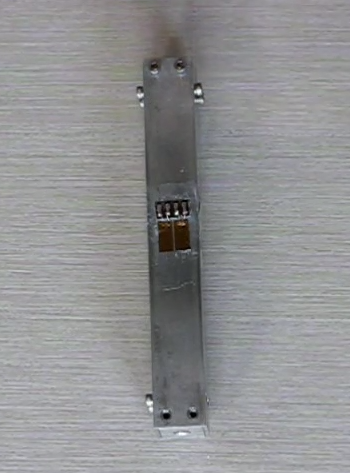
\includegraphics[width=0.4\columnwidth]{figs/forca/1.png}
    \caption{Exemplo de um sensor de força: cilindro com strain gauge acoplado.}
    \label{forca_1}
\end{figure}


 A resistência elétrica de um fio varia conforme seu comprimento e sua área, portanto, a variação de corrente que passa por este fio pode ser utilizada como medida quantitativa e é possível determinar a força aplicada por um modelo matemático conhecido: $R=\frac{\rho L}{A}$. Outros sensores que poderiam atender às especificações, mas são de mais difícil comercialização, em relação aos requisitos de projeto, são: sensor de força piezoelétrico

 De acordo com \textbf{Guide to the Measurement of Force}, a aplicação pode ser caracterizada como sistema para medições e controle de forças para operações de segurança. Pode ainda ser especificada como \textbf{Crane overload/underload protection}, que consiste em monitorar forças atuando em garras tipo pescadora ou gancho (ver figura~\ref{forca_2}), no qual a medida será avaliada em situações estáticas ou de pouco movimento/vibração.

  \begin{figure}[H]
    \centering
    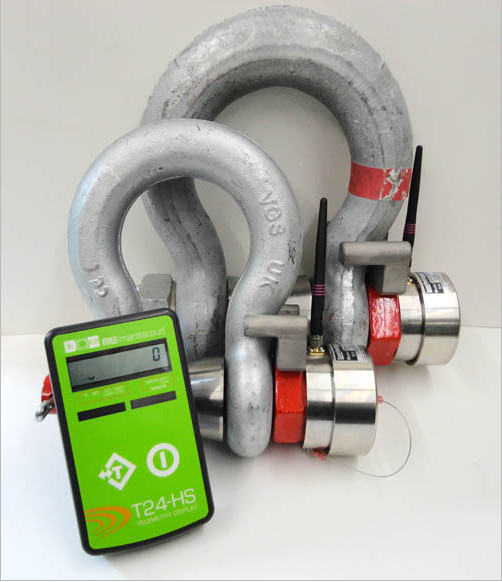
\includegraphics[width=0.4\columnwidth]{figs/forca/2.png}
    \caption{Exemplo de instalação de sensor de força em garra.}
    \label{forca_2}
\end{figure}

A solução por sensores de força é eficiente em aplicações onde se deseja avaliar frequência de vibração e duração da onda de choque, porém não muito na medida quantitativa e comparativa de forças devido à sensibilidade do strain gauge a campos magnéticos externos, pressão hidrostática e umidade. A variação de acúmulo de sedimentos no stoplog também dificulta a calibração do instrumento.

Os fornecedores para sensores de força do tipo strain gauge avaliados nesta pesquisa são: Applied Measurements Limited, Load Cell Central, Transducer Techniques. Os modelos avaliados são da série DBEP e CLP de seus respectivos fornecedores.


%%%%%%%%%%%%%%

\subsubsection{Sensor indutivo de proximidade}

Sensores indutivos de proximidade podem ser utilizados para detectarem a presença da garra pescadora. Este sensor de presença pode ser do tipo linear, podendo ser realizada análise quantitativa, ou simplesmente chaveado, um simples indicador de presença. Portanto, pode indicar encaixe mal ou bem sucedido durante a operação de remoção/inserção de stoplogs. Os sensores indutivos apresentam a mesma forma de operação nos diversos produtos disponíveis no mercado, diferenciando-se principalmente na medida de distância da aplicação.

 O sistema para sensoriamento por indução magnética é composto por uma fonte de alimentação e um indutor. Ao alimentar o sensor indutivo, uma corrente alternada é gerada. A corrente elétrica que passa pelo indutor gera um campo magnético na face do sensor. Este campo magnético induz corrente de Foucault no alvo metálico, que aumenta conforme o alvo se aproxima do sensor indutivo. O aumento das correntes de Foucault cria um campo magnético no alvo, que irá se opor ao campo produzido pelo sensor indutivo. Essa redução do campo magnético pode ser medida e, portanto, é possível presenciar o alvo.

 Existem diversos sensores indutivos disponíveis no mercado que atendem às especificações, apresentam o mesmo modo de operação e diferenciam-se principalmente quanto à robustez, instalação (faceada ou não) e interface de saída. A resistência a choques, vibração, submersibilidade e o tipo de instalação são as características mais importantes para a aplicação. O sensor deve ser do tipo IP69K e faceado, o que diminui o alcance, mas aumenta a proteção.

 A pesquisa por sensores indutivos de proximidade para a finalidade desejada resultou em aplicações equivalentes. A empresa \textbf{HATCH - Energy Innovations} desenvolveu em 2007 um Lifting Beam instrumentado com sensores indutivos (ver figura~\ref{indutivo_1}). Em 2008, a empresa \textbf{Atlas Polar} adotou a mesma solução com sensores indutivos.

 \begin{figure}[H]
    \centering
    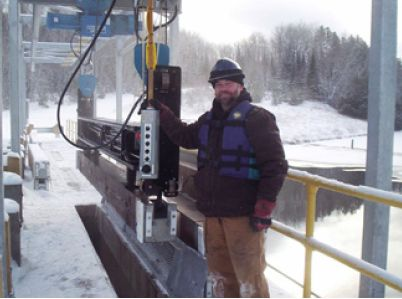
\includegraphics[width=0.5\columnwidth]{figs/indutivo/1.jpg}
    \caption{Lifting Beam desenvolvido pela empresa HATCH}
    \label{indutivo_1}
\end{figure}

A solução por sensores indutivos é eficiente em aplicações onde se deseja avaliar a presença de stoplog. A grande maioria dos sensores são frágeis a choque e vibração, além de sensíveis a ruídos elétricos e magnéticos. Porém, já há no mercado produtos IP69K e encapsulados. Há, também, a possibilidade de falso positivo em caso de sedimentos metálicos, mas é baixa a probabilidade.
Pesquisas em aplicações semelhantes mostraram que o sensor indutivo é a solução adotada para o monitoramento de encaixe entre garra pescadora e stoplog, auxiliado por outros sensores ou sistemas independentes de atuadores.

Os fornecedores pesquisados para sensores indutivos que atendem aos requisitos de projeto são: Contrinex, Pepperl-Fuchs, Positek e Turck. Diversos modelos foram avaliados, juntamente com os técnicos das respectivas empresas.

%%%%%%%%%%%%%%

\subsubsection{Sensor capacitivo de proximidade}
Os sensores capacitivos de proximidade são capazes de detectar objetos devido à capacidade destes alvos em serem carregados eletricamente. Analogamente ao sensor indutivo, que detecta variações de campo magnético devido a alvos metálicos, o sensor capacitivo é sensível a variações na capacitância (ver figura~\ref{capacitivo_1}).

\begin{figure}[H]
    \centering
    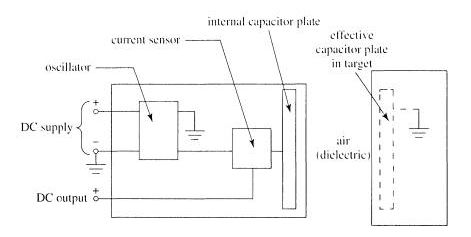
\includegraphics[width=0.8\columnwidth]{figs/capacitivo/1.jpg}
    \caption{Sensor capacitivo}
    \label{capacitivo_1}
\end{figure}

Internamente ao sensor, há um circuito que utliza a alimentação DC para gerar voltagem alternada (oscilador). O circuito interno RC é, então, alimentado e uma corrente alternada passa por esse circuito. O fluxo de corrente alternada depende da capacitância, e esta varia  conforme a distância e área entre as placas do capacitor e o material dielétrico entre as placas: $C = \frac{\epsilon A}{d}$.

Em sensores capacitivos, uma placa do capacitor está no sensor e a outra é o objeto a ser detectado, que pode ser um material metálico ou não-metálico. A aproximação do alvo modifica a capacitância, resultando em variações no campo elétrico e na corrente alternada. Finalmente, as variações da corrente podem ser medidas e o alvo é detectado.

As características que devem ser avaliadas em sensores capacitivos são as mesmas dos sensores indutivos, como tipo de instalação, modo de operação chaveado ou linear e etc. Porém, deve-se atentar ao fator de redução, que depende do alvo a ser detectado.

 Os sensores capacitvos exercem função semelhante ao sensor indutivo e pode ser utilizado para detecção de presença de stoplog. Porém, a calibração se mostra bem mais complexa devido à sensibilidade do sensor e ao fato de não estar restrito a detecção de materiais metálicos. A chance de falsos positivos será bem maior em caso de escolha deste sensor em comparação com o sensor indutivo.


Os fornecedores pesquisados de sensores capacitivos que atendem aos requisitos de projeto são: Contrinex, Pepperl-Fuchs, Positek e Turck. Diversos modelos foram avaliados, juntamente com os técnicos das respectivas empresas.

%% ***************


 \subsubsection{Conclusão de análise técnica}\mbox{}\\


As tecnologias que foram analisadas para detectar o contato entra a garra pescadora e o Stoplog foram: sensor de força, sensor indutivo e sensor capacitivo. Os sensores de força necessitaria de ser instalados nos eixos da garra pescadora, logo alterando a estrutura mecânica do mesmo, além de serem sensíveis a calibração, logodesconsiderados como uma solução viável. O sensor capacitivo, assim como o sensor indutivo, podem ser instalados diretamente na garra pescadora, entretanto o capacitivo não está restrito a detecção de materiais metálicos, logo resultaria em maiores chances de falsos positivos que os sensores indutivos.  Sendo assim, a solução de medição de contato por sensor indutivo se mostra mais eficiente para a detecção do contato entre a garra pescadora e o Stoplog. 

Dados os requerimentos do meio foi buscado no mercado produtos a prova d’agua e encapsulados com nível de proteção mínima IP69K. Os fornecedores pesquisados para sensores indutivos que atendem aos requisitos de projeto são: Contrinex, Pepperl-Fuchs, Positek e Turck. Diversos modelos foram avaliados, juntamente com os técnicos das respectivas empresas. A lista dos modelos de cada fabricante que seriam ideais à aplicação no projeto se encontra na tabela abaixo. Por os modelos serem equivalente em aplicabilidade, foi selecionado o sensor que apresenta o menor custo ao projeto o NBB20-L2-E2-V1 de instalação faceada, chaveado normalmente aberto e distância de operação de 2cm (figura~\ref{indutivo_1}).


\begin{center}
    \begin{tabular}{| l | l | l | l | }
    \hline
	{\bf Modelo} & 	{\bf Fabricante} &		{\bf Distribuidor}	&	{\bf Preço} \\  \hline
	DW-LD-M18&		Contrinex&			Electric Control&		428,97 R{\$} \\  \hline
	NBB20&			Pepperl-Fuchs&		Pepperl-Fuchs Brasil&	181,17 R{\$} \\  \hline
	NI35&			TURCK&				TURCK Brasil&			514,29 R{\$} \\  \hline
	NI50-Q42&		TURCK&				TURCK Brasil&			414,75 R{\$} \\ \hline
\hline 
\end{tabular}
\end{center}

\begin{figure}[H]
    \centering
    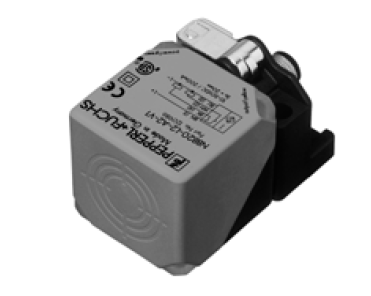
\includegraphics[width=0.4\columnwidth]{figs/indutivo/1.png}
    \caption{Sensor indutivo do fornecedor Pepperl-Fuchs.}
    \label{indutivo_1}
\end{figure}